

\documentclass[twoside,twocolumn]{article}

\usepackage{blindtext} % Package to generate dummy text throughout this template 

\usepackage[sc]{mathpazo} % Use the Palatino font
\usepackage[T1]{fontenc} % Use 8-bit encoding that has 256 glyphs
\linespread{1.05} % Line spacing - Palatino needs more space between lines
\usepackage{microtype} % Slightly tweak font spacing for aesthetics

\usepackage[english]{babel} % Language hyphenation and typographical rules

\usepackage[hmarginratio=1:1,top=32mm,columnsep=20pt]{geometry} % Document margins
\usepackage[hang, small,labelfont=bf,up,textfont=it,up]{caption} % Custom captions under/above floats in tables or figures
\usepackage{booktabs} % Horizontal rules in tables

\usepackage{lettrine} % The lettrine is the first enlarged letter at the beginning of the text
\usepackage{todonotes}
\usepackage{enumitem} % Customized lists
\setlist[itemize]{noitemsep} % Make itemize lists more compact

\usepackage{abstract} % Allows abstract customization
\renewcommand{\abstractnamefont}{\normalfont\bfseries} % Set the "Abstract" text to bold
\renewcommand{\abstracttextfont}{\normalfont\small\itshape} % Set the abstract itself to small italic text

\usepackage{titlesec} % Allows customization of titles
\renewcommand\thesection{\Roman{section}} % Roman numerals for the sections
\renewcommand\thesubsection{\roman{subsection}} % roman numerals for subsections
\titleformat{\section}[block]{\large\scshape\centering}{\thesection.}{1em}{} % Change the look of the section titles
\titleformat{\subsection}[block]{\large}{\thesubsection.}{1em}{} % Change the look of the section titles

\usepackage{fancyhdr} % Headers and footers
\pagestyle{fancy} % All pages have headers and footers
\fancyhead{} % Blank out the default header
\fancyfoot{} % Blank out the default footer
\fancyhead[C]{Persistent Homology of Adversarial Images} % Custom header text
\fancyfoot[RO,LE]{\thepage} % Custom footer text

\usepackage{titling} % Customizing the title section

\usepackage{hyperref} % For hyperlinks in the PDF

\usepackage{graphicx} % For importing images
\usepackage{subfig}

\usepackage{algorithmic} % For pseudocode
\usepackage{algorithm}

\usepackage{amsmath}
\DeclareMathOperator{\sign}{sign} 

%----------------------------------------------------------------------------------------
%	TITLE SECTION
%----------------------------------------------------------------------------------------

\setlength{\droptitle}{-4\baselineskip} % Move the title up

% \pretitle{\begin{center}\Huge\bfseries} % Article title formatting
% \posttitle{\end{center}} % Article title closing formatting
\title{\LARGE Persistent Homology of Adversarial Images} % Article title
\author{%
\textsc{Edric Tam}\\[1ex] % Your name
\normalsize Duke University \\ % Your institution
\normalsize \href{mailto:edric.tam@duke.edu}{edric.tam@duke.edu} % Your email address
\and % Uncomment if 2 authors are required, duplicate these 4 lines if more
\textsc{Craig Chen}\\[1ex] % Second author's name
\normalsize Duke University \\ % Second author's institution
\normalsize \href{mailto:craig.chen@duke.edu}{craig.chen@duke.edu} % Second author's email address
}
\date{\today} % Leave empty to omit a date
\renewcommand{\maketitlehookd}{%
\begin{abstract}
\noindent 
It is now known that even the most well-trained and generalizable image-classification neural network models can succumb to adversarial attacks. To the human eye, the adversarial image may be indistinguishable from the original, but to the machine learning model, they are of two different classes. Existing approaches have shown that this weakness seems to be related to the inherent structure of artificial neural nets. Our analysis, through zero and one dimensional persistence diagrams, shows that there is also a noticeable difference between the original and adversarial images. Furthermore, the persistence diagrams of adversarial noise differ from that of Gaussian noise.
\end{abstract}
}

%----------------------------------------------------------------------------------------

\begin{document}

% Print the title
\maketitle

%----------------------------------------------------------------------------------------
%	ARTICLE CONTENTS
%----------------------------------------------------------------------------------------

\section{Introduction}

\lettrine[nindent=0em,lines=3]{D} eep learning is a rapidly developing area of machine learning that has made huge changes to how technology affects our daily lives. From image classification to computer vision, reinforcement learning to natural language processing, deep neural networks have achieved state-of-the-art performances that far exceeds that of other machine learning models, sometimes even surpassing humans in accuracy and speed on these tasks. These advancements have led to very wide adoption in industrial applications, e.g. logging in via face recognition on mobile phones, using fingerprints to authenticate users to applications etc. This means that the security aspect of these Deep Learning algorithms, traditionally an under-studied subject, is crucial to ensure that the privacy and safety of the billions of users using these technologies. 

It is now known that even the most well-trained and generalizable image-classification neural network models can succumb to adversarial attacks. To the human eye, the adversarial image may be indistinguishable from the original, but to the machine learning model, they are of two different classes. Existing research shows that the existence of adversarial examples are not specific to neural networks in the image classification settings. Adversarial examples also exist in many kernel-based machine learning methods such as support vector machines, and manifest themselves in applications with text data, language data etc. However, due to the visual nature of image classification tasks, we have adopted the standard MNIST benchmark for our experiments to better illustrate the concepts underlying this paper. However, note that similar extensions to other machine learning models involving image recognition should be straightforward. 

We mainly conduct our experiments through the lens of computational topology. In particular, we have focused our analysis on the zero- and one-dimensional persistence diagrams of the original/adversarial images. We also compare the topological structure of these adversarial perturbations against those that arise from more natural distributions, such as the Gaussian. Our results show that not only are there visually discernible differences in the persistence diagrams of natural and adversarial noise, there are also statistical testing methods can potentially capture these differences.

We hope that this report would illuminate future work in similar directions. 

In section 2, we outline the prerequisite background knowledge in adversarial images as well as persistent homology needed for understanding the paper. In section 3, we describe the methods that we adopted in our experiments. In section 4, we list our results as well as related figures. In section 5, we discuss the interpretation of these results as well as potential future directions. 

%------------------------------------------------

\section{Preliminaries and Background}

\subsection{Adversarial Images}

Most of the existing mainstream methods in the literature generate adversarial images with 2 input ingredients: 
\begin{itemize}
    \item the original dataset (images,labels)
    \item a trained classifier
\end{itemize}
In this paper, the classifier that we will consider will be a pre-trained neural network, not a black-box model. In other words, we have "oracle" access to the classifier and its parameters. In real life settings, attackers generally don't have access to the true classifier; however, due to certain intriguing "universality" results, adversarial images generated from one model generally work for a wide range of classifiers that fall into the same category of network architecture. Hence, having "oracle" access to the true classifier is not an essential requirement, but we have chosen this setup for simplicity. 

There are multiple ways to generate adversarial images for neural networks, and recent work has shown that even 1-pixel changes can be sufficient to deceive machine learning models. In this report, we stick to the basics and use two related techniques: the Fast Gradient Sign Method (FGSM) \cite{goodfellow2014} and the similar gradient-based optimization approach \cite{szegedy2013}.

In the Fast Gradient Sign method, we take an original image, say a "1" in MNIST, and add noise to perturb it so that the classifier would misclassify it to another label, say a "7". This is achieved by taking the gradient of the cost function of the classifier with respect to the input data, and adding it to the original image. The intuition for why this works is as follows: typically, machine learning models aim to minimize a certain loss function in order to maximize classification accuracy. In this FGSM scenario, we are adding the noise in the direction of the gradient that maximizes the loss function, thus causing the mislabeling. Explicitly, we generate the adversarial image $x'$ as follows:
$$
x' = x + \varepsilon \sign (\nabla_x L(x,y))
$$
where $x$ is the original input, $y$ is the true label of $x$, and $L$ is the loss function.

In the second technique, an adversarial perturbation is generated by running an optimization algorithm on the \emph{input} vector so that it minimizes a target loss function. In this paper, we perform gradient descent on a randomly initialized input vector with respect to the loss function: 
$$
C(x) = \frac{1}{2} \Vert y_{goal} - y(x) \Vert^2
+ \lambda \Vert x_{mimic} - x \Vert^2
$$  
where $x$ is the input vector, $y_{goal}$ is the label output we desire, $x_{mimic}$ is the appearance we seek to mimic, and $y(x)$ is the output of the classifier. $\lambda \in [0,\infty)$ is a hyperparameter that is typically set to 0.05 - the larger the value, the more we want to prioritize the appearance of the input. 

\subsection{Persistent Homology}

\begin{figure*}
    \centering
    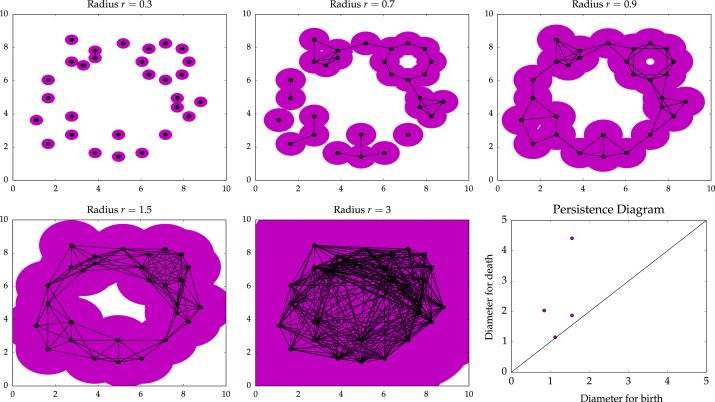
\includegraphics[scale=0.55]{figures/pers_hom_example.jpg}
    \caption{The gradual thickening of a point cloud in $\mathbb{R}^2$ and the 1-dim Persistence Diagram.}
    \label{fig:pers_hom_example}
\end{figure*}

There are many ways to computationally and visually examine the topology of certain objects/data. For a general treatment, we refer readers to the excellent text by Edelsbrunner and Harer \cite{edelsbrunnerharer}. For this analysis, we will focus on a particular aspect called Persistent Homology, especially in 0-D and 1-D. 

Intuitively, for 0-D persistent homology in Euclidean space, we are primarily focusing on the connected components in the object under examination. The way we achieve that is by "growing balls" around each point in the object, and noting when they "touch"/merge. The "birth"/"death" of these components are tracked through time, and can be presented visually in the form of a persistent diagram. 

We do something very similar for 1-D persistent homology, where we still consider growing balls around each point, except that time time rather than tracking the birth and death of connected components, we track the birth and death of loops instead. For an example of the \v Cech complex of a given point cloud as the radius grows, see Figure \ref{fig:pers_hom_example}. 


\section{Methods}

\subsection{Dataset and Setup}
We have adopted the popular benchmark image classification dataset MNIST for our experiments. It consists of 60000 training images and 10000 testing images. Each of the digits, ranging from 0 to 9, represents one-tenth of the data in the dataset. In general, a very simple feed-forward neural network, under relatively little training (e.g. 10 epochs) could achieve a testing accuracy of around 95 percent in this dataset. 

It is worth noting that the "victim" neural net in our experiments is a fully connected multi-layer neural network. If one is to repeat this work with a convolutional neural network, we expect that the adversarial images produced may yield persistence diagrams that differ from ours.

\subsection{Adversarial Noise}
We first performed adversarial image generation using the FGSM method outlined above, adopting and modifying code from a tutorial available on the PyTorch website \url{https://pytorch.org/tutorials/beginner/fgsm\_tutorial.html}. A random sample of the generated adversarial images are displayed in Figure \ref{fig:adversarialgenerated}. Several characteristics are of note: 
\begin{itemize}
    \item[1)] 
    Even with very small, visually imperceptible perturbations (e.g. $\epsilon = 0.05$) to the images, the network could be fooled. 
    \item[2)]
    As the noise levels become higher, the noises in the images become more apparent, with certain "patchy" patterns emerging (see Figure \ref{fig:adversarialgenerated}).   
\end{itemize}

\subsection{0-D Persistent Homology}

Given the visual "patchy" patterns of the adversarial images generated using FGSM, it is natural to consider a 0-D persistent homology analysis of the images, which tracks the birth and death of connected components. In Figure \ref{fig:persistenceAdv}, in the top figure we plot an example adversarial image side by side with its 0-D persistent homology diagram. While this is certainly interesting and useful, note that it is likely that the filtration diagram captured the a lot of the structure of the digit itself, which is very pronounced in the adversarial image. Since our interest mainly lies in the adversarial noise rather than the structure of the digit itself, in the middle row we filtered out the noise component of the adversarial image using a high-pass filter, so that the high frequency adversarial noisy components would be retained and the effect of the digit structure would be alleviated. As a control, we added gaussian white noise of similar L2 magnitude to the original image, and applied the same high-pass filter. Resulting plots of the corresponding filtration diagrams now show clear visually discernible patterns. In general, we observe that adversarial noises are more structured and thus has fewer points appearing on the persistence diagram, whereas i.i.d. gaussian noise is less structured, resulting in many more components and points. 

\subsection{Statistical Testing}

The above analysis, while promising and interesting, is of a visual and exploratory nature. We would like to potentially automate the testing of adversarial noise versus i.i.d. distributed Gaussian noise via a more objective procedure that could be automatically applied. In order to perform statistical testing, we need several ingredients. First, we need the "size" of the test, typically set at $0.05$. Second, we need a test statistic. There are many potentially interesting ways of picking this, and here we focus on a popular topological metric called the average lifetime. It represents the average lifetime of the connected components tracked. Last but not least, we need a null distribution of the test statistic. Here, we generate the null-distribution via a generative approach. We calculate the average lifetime of (say 100) different draws of the Gaussian noise, and then compare the actual adversarial noise that we obtain to that empirical distribution. If the average lifetime of the adversarial noise lies within the top 2.5 percent or bottom 2.5 percent of the empirical distribution, then we would reject the null hypothesis. In Figure \ref{fig:testing} below, we outline two example cases, where in the first case we failed to reject the null and in the second case we reject the null. 

In trying this approach, it is found that the efficacy and robustness of this test largely depends on the sizes of the noise applied. If we manually adjust the variance parameter of the simulated Gaussian noise so that the L2 norm of the Gaussian noise in the null and the adversarial noise are matched exactly to several decimal points, then in general the test can pick up differences between the average lifetime of the Gaussian noises in the null distribution and the adversarial noises. 

However, if the sizes of the noises are even slightly different, i.e. we test against Gaussian noises that have a variance parameter that differs from the null's variance parameter by just $0.01$, then the test often rejects the null hypothesis. This implies that the test would frequently result in false negatives if the variance parameter of the null distribution is not calibrated properly, since the average lifetime analysis would then be capturing the sizes of the noise in addition to the structure of the noise.  Note that in reality, we often do not know the appropriate noise level exactly and would have to estimate/guess the noise level, and some approximation error in the appropriate noise/variance level would be inevitable. This means that we would need to improve upon the false-negative accuracy of this test in future studies or have access to very accurate noise levels in order for this test to be useful in reality.



\begin{figure*}[!htb]
    
	\centering
	\subfloat[Adversarial Images generated from FGSM]{
	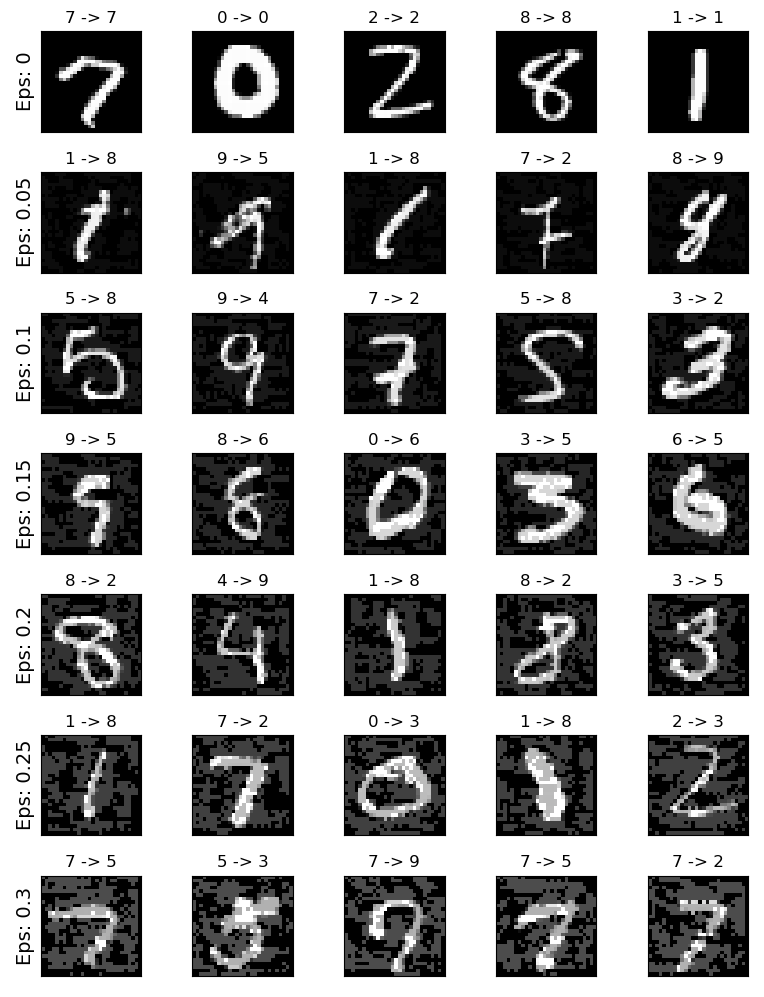
\includegraphics[scale=0.5]{figures/adversarial.png}}

	
	\caption{A random sample of generated Adversarial images using FGSM. Each row represents a different noise level, with the labels before and after the perturbation noted. Generated by code adopted and modified from Pytorch FGSM tutorial.}
	\label{fig:adversarialgenerated}
\end{figure*}

\begin{figure*}[!htb]
    
	\centering
	\subfloat[Adversarial image]{
	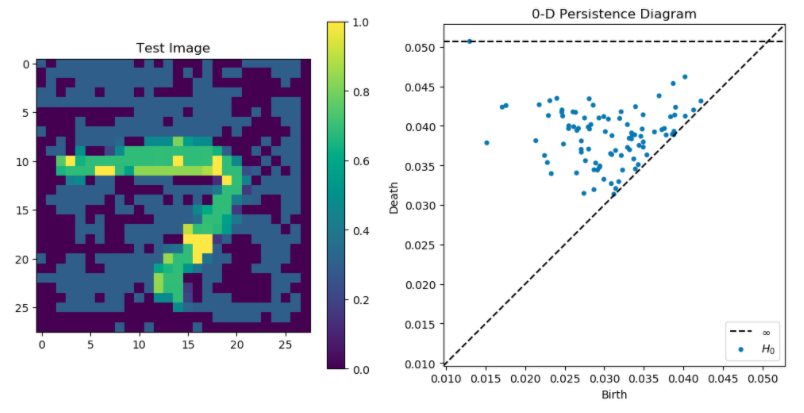
\includegraphics[scale=0.5]{figures/advimage.png}}\\
	\vspace{-1.2em}
	\subfloat[Adversarial Noise (obtained by applying high pass filter)]{
	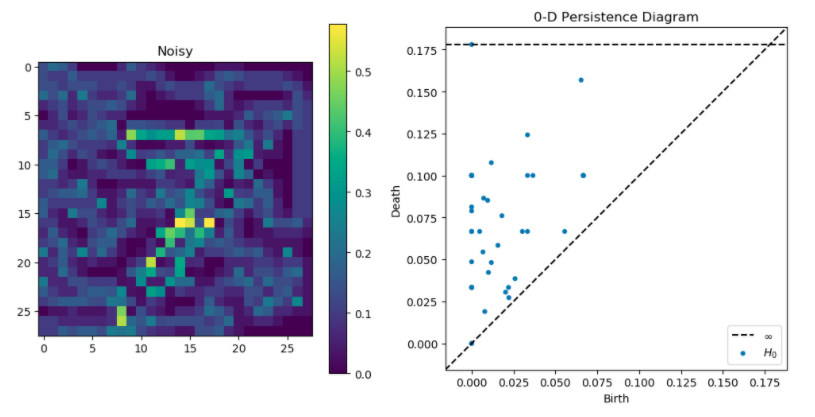
\includegraphics[scale=0.5]{figures/advnoise.png}}\\ 
	\vspace{-1.2em}
	\subfloat[Gaussian Noise (obtained by applying high pass filter)]{
	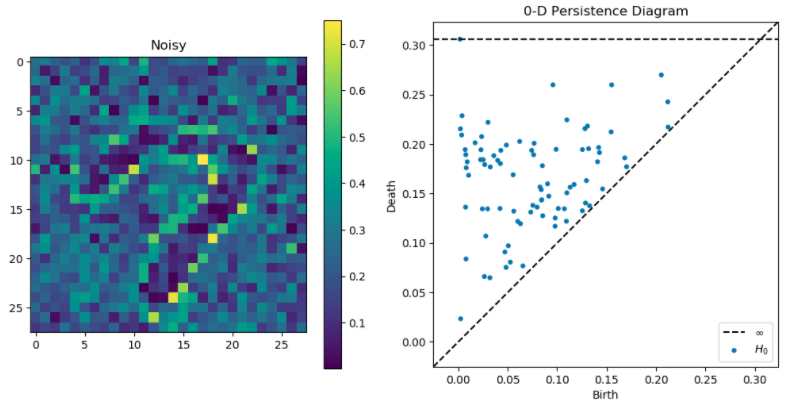
\includegraphics[scale=0.5]{figures/newadv.png}}
	\caption{ }
	\label{fig:persistenceAdv}
\end{figure*}

\begin{figure*}[!htb]
    
	\centering
	\subfloat[A case where we fail to reject the null]{
	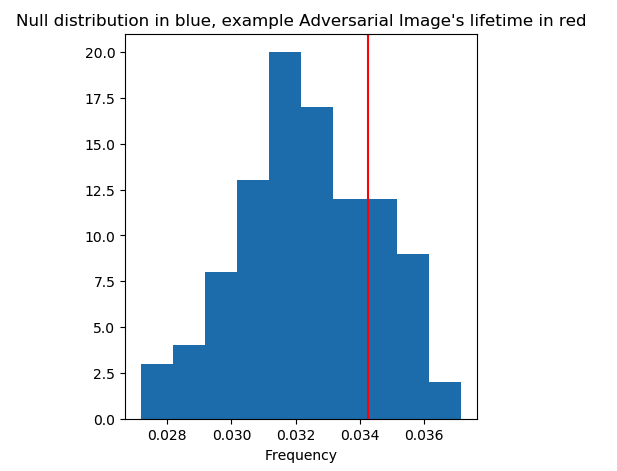
\includegraphics[scale=0.5]{figures/failrej.png}}\\ 
	\vspace{-1.2em}
	\subfloat[A case where we reject the null]{
	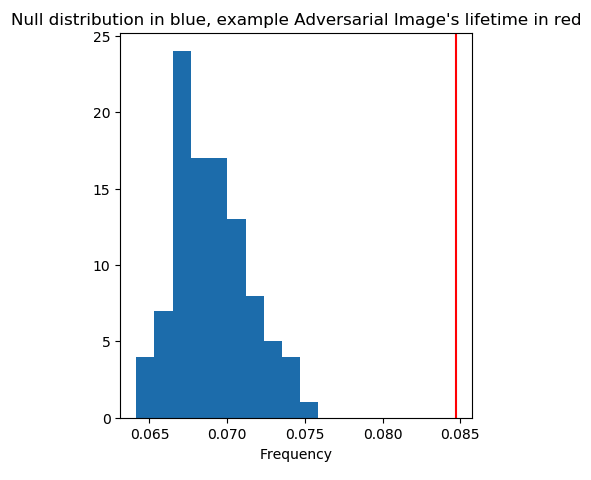
\includegraphics[scale=0.5]{figures/reject.png}}
	\caption{ }
	\label{fig:testing}
\end{figure*}

\subsection{Targeted Attacks}

In contrast to the FGSM, the process of generating a targeted adversarial image specifies exactly which label we want the pre-trained network to misclassify our image as - this is the $y_{goal}$ term in the loss function. We used Algorithm 1 to produce the targeted adversarial images.

\begin{algorithm}
\caption{Generate targeted adv. image}
\begin{algorithmic}
\STATE Input: target label $y_{goal}$, mimic label $x_{mimic}$
\STATE Input: hyperparameters ($\lambda$, $\alpha$, K epochs)
\STATE Input: Pre-trained classifier
\STATE Initialize $\vec{x}$ entries i.i.d. $N(0,1)$
\FOR{i = 1,...,K}
    \STATE compute $\nabla_x C(x)$
    \STATE $x \gets x - \alpha \nabla_x C(x)$
\ENDFOR
\RETURN $x$
\end{algorithmic}
\end{algorithm}


Then, we transform the images into a 3D point cloud where the $x$ and $y$ coordinates correspond to the row and column of the pixel, respectively, and the $z$ value is brightness of the pixel. The $x,y$ values are then normalized so that the point cloud exists inside the unit cube since the brightness values are pre-normalized from the data set. 

This array of points is then inputted into Ripser where the 0 and 1-dim persistent homology is determined via Rips filtration. For an example, see Figure \ref{fig:targetedcomparison}.

%------------------------------------------------

\begin{figure*}[!htb]
    
	\centering
	\subfloat[Mimic Image]{
	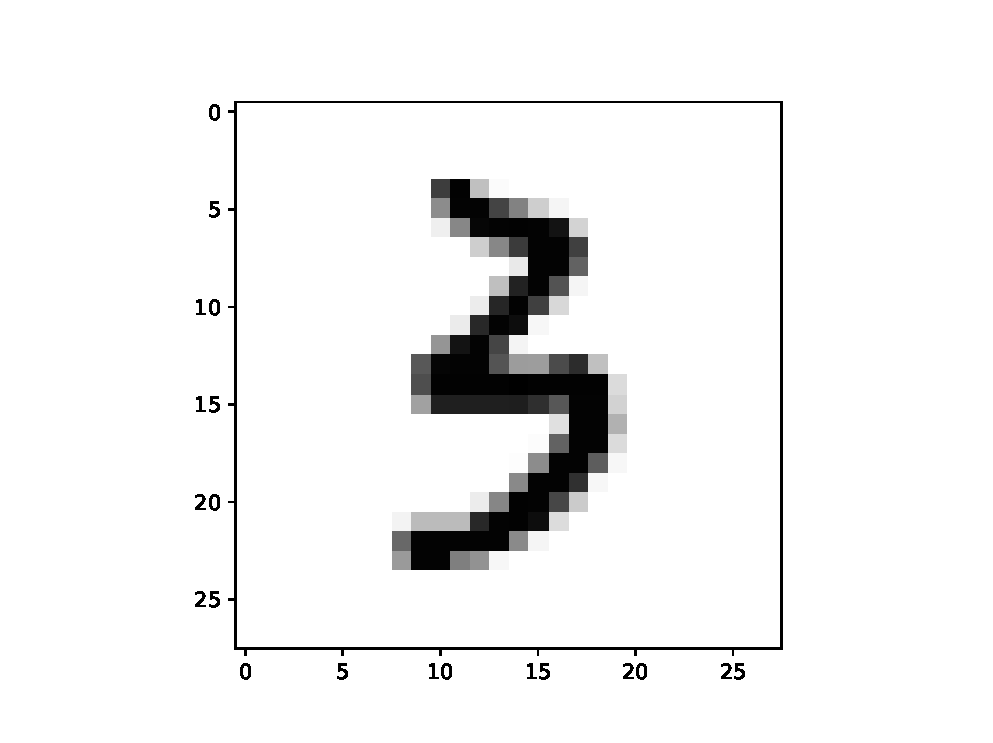
\includegraphics[scale=0.5]{figures/mimic3.eps}}
	\subfloat[Persistence Diagram of the mimic image]{
	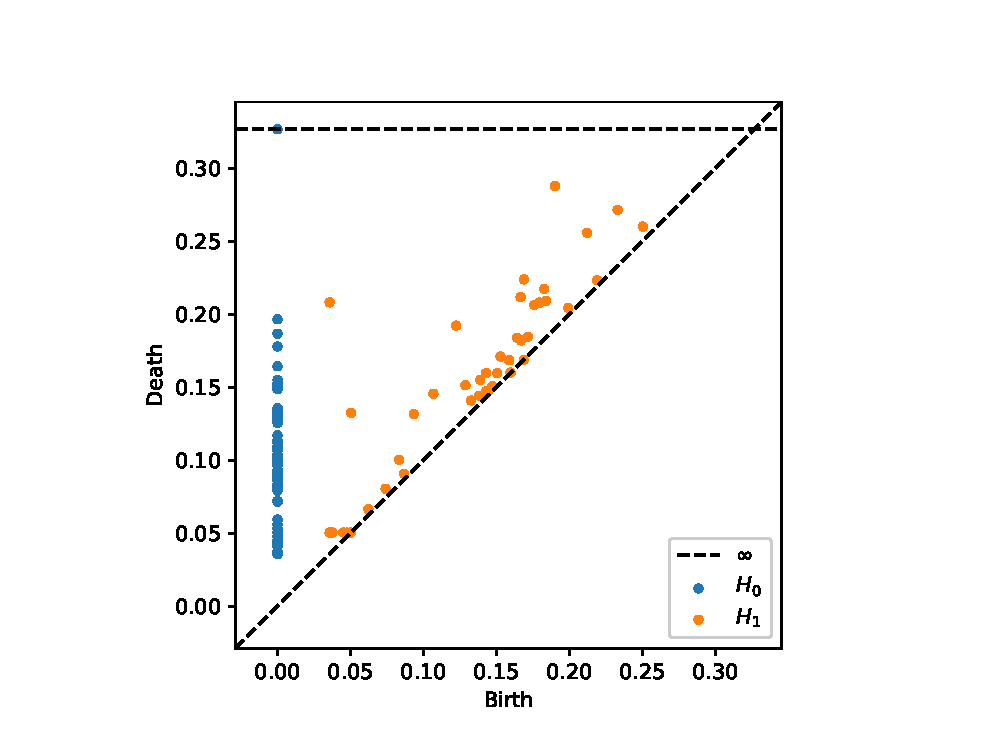
\includegraphics[scale=0.5]{figures/persdgm_mimic3.eps}}
	\\
	\vspace{-1.2em}
	\subfloat[Adversarial Image, results in classification as 6]{
	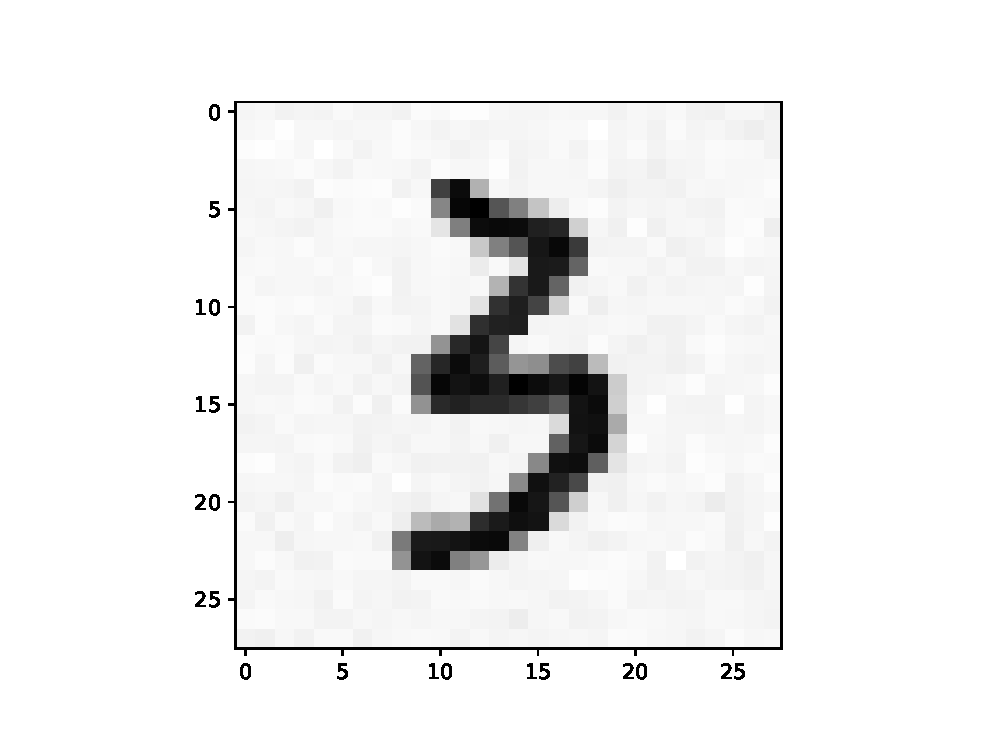
\includegraphics[scale=0.5]{figures/adversarial3.eps}}
	\subfloat[Persistence Diagram of the adversarial image]{
	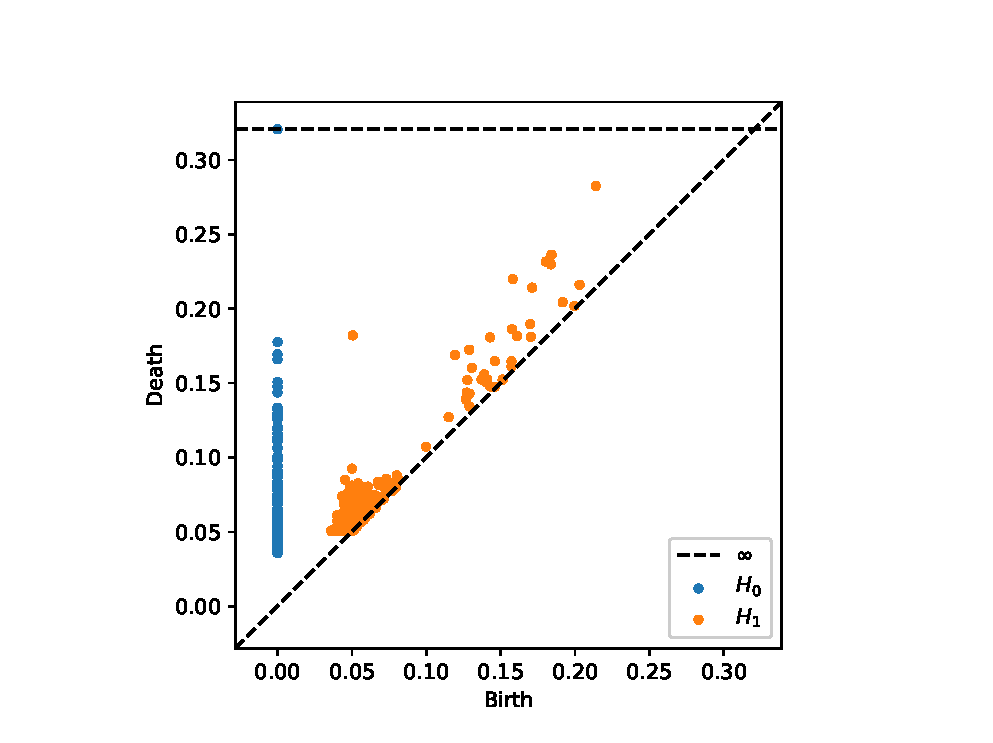
\includegraphics[scale=0.5]{figures/persdgm_adversarial3.eps}}
	\\ 
	\vspace{-1.2em}
	\subfloat[Noisy Image]{
	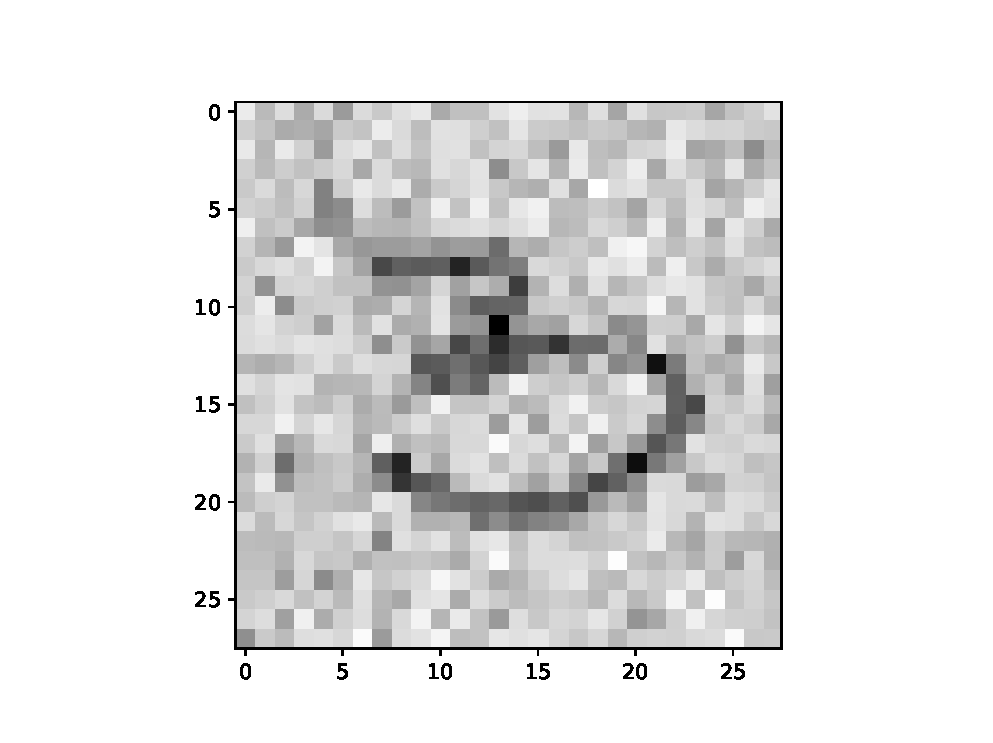
\includegraphics[scale=0.5]{figures/noisy3.eps}}
	\subfloat[Persistence Diagram of the noisy image]{
	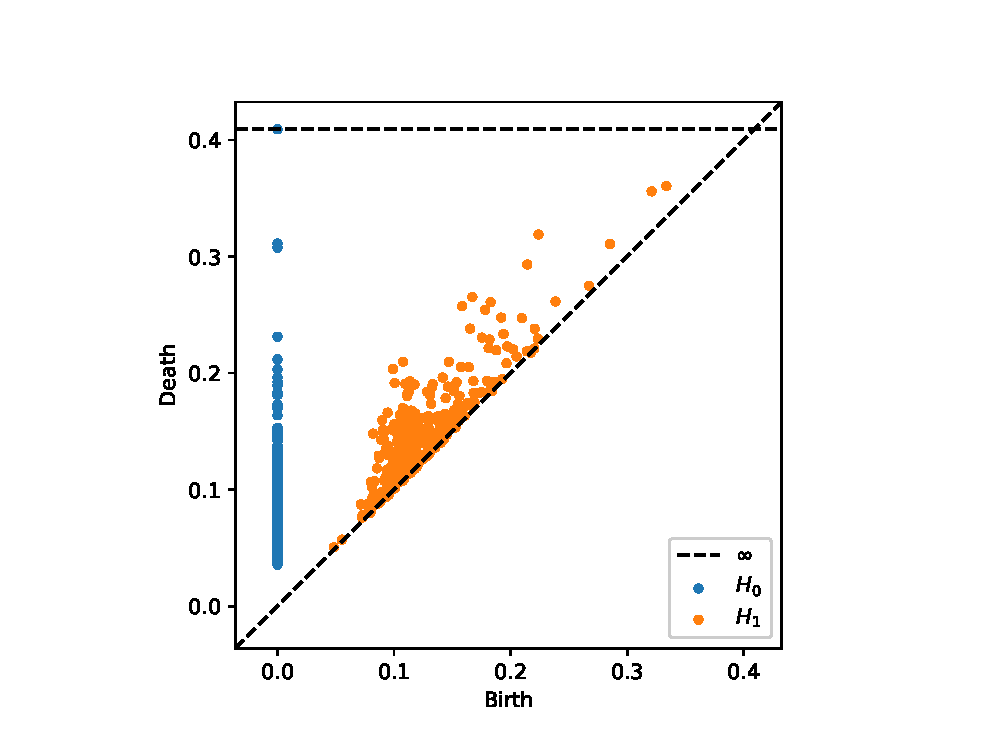
\includegraphics[scale=0.5]{figures/persdgm_noisy3.eps}}
	
	\caption{Persistence Diagrams of Three Types of Images.\\
	(a),(b) A "3" from the MNIST dataset and its 0,1-dim persistence diagrams. \\
	(c),(d) An adversarial image generated using gradient descent on a random input with parameters:\\
	    \-\hspace{1em} $x_{mimic} = (a), y_{goal} = 6, \lambda = 0.05, \alpha = 0.05, K = 1000$. 
	\\
	(e),(f) Image (a) with additive entry-wise N(0,0.05) noise and corresponding persistence diagram.}
	\label{fig:targetedcomparison}
\end{figure*}

\section{Results}

From our experiments, we found that there is a noticeable visual difference between the topological properties of adversarial images, their original counterparts, and noise-added variants. For both the untargeted and targeted methods of generating adversarial images, we observe that the resulting images tend to preserve many of the topological structures of the original images. To us, this serves as a visual indicator that there is something inherently different that sets the adversarial noise apart from standard i.i.d gaussian noise. 

Figure \ref{fig:persistenceAdv} provides a sample for what the 0-D persistence diagrams pick up in comparing the adversarial image, the adversarial noise and the gaussian noise. It is clear in this case (and in general) that in the 0-D persistence diagram the adversarial noise show a sparser pattern and are closer to the original when compared to i.i.d. gaussian noise.  While this is of a more visual nature, Figure \ref{fig:testing} provides two plots that illustrate the statistical testing approach we adopted.  We ran this test multiple times and observed that for the vast majority of trials, the test results in rejection of the null, regardless of whether the noise is Gaussian or adversarial, mainly because the test is sensitive to the noise level of the null.

Figure \ref{fig:targetedcomparison} depicts the differences between the persistence diagrams the targeted adversarial image and the other classes of images we are interested in. Immediately one notices the clumps of points in the adversarial and noisy 1-D persistence diagrams that are absent in the diagram of the original image. There is also a qualitative difference between the shape of the clumps in the adversarial and noisy images - the clumps appear to be similarly cone-shaped but differ in size. One could imagine that the size of the clumps in the noisy image can be controlled by adjusting the standard deviation of the added noise, and this may in fact be the case.

Perhaps more interestingly, the persistence diagram of the adversarial image appears to contain more features of the original image whereas the noise-added image appears to have "lost" many features. Here, we use features in a very general sense to discuss the appearance of the 1-D persistence diagrams. This may seem like an obvious difference as during the process of generating the adversarial image there is an incentive to mimic the original image; however, it is not immediately obvious that the inclusion of adversarial perturbations should not alter the 1-D homology of the image.

%------------------------------------------------

\section{Conclusion and Discussion}

Despite yielding some interesting results, our work leaves a lot to be desired. The results may appear compelling to the human eye, but more rigorous methods are needed to determine whether or not there is a significant difference between the persistence diagrams of the adversarial images.

\textbf{Future Work}: It may be interesting to feed the persistence diagrams of the original, adversarial, and noisy images into another machine learning model. It seems likely that there is a classifiable difference between the persistence diagrams yielded by the three types of images. Additionally, the same line of analysis may yield more interesting results when applied to a convolutional neural net, rather than the simple fully-connected net used to produce our results. Furthermore, it is known that the MNIST digits dataset is rather easy for machine learning models to learn. Experiments with more challenging data sets and higher resolution images are a clear way forwards to improve upon our results.



%----------------------------------------------------------------------------------------
%	REFERENCE LIST
%----------------------------------------------------------------------------------------

\begin{thebibliography}{99} % Bibliography - this is intentionally simple in this template

\bibitem[1]{goodfellow2014}
\textbf{Goodfellow et al.}
\newblock Explaining and Harnessing Adversarial Examples. 2014.
\newblock {\em International Conference on Learning Representations}, https://arxiv.org/abs/1412.6572

\bibitem[2]{szegedy2013}
\textbf{Szegedy et al.}
\newblock Intriguing properties of neural networks. 2013.
\newblock {\em International Conference on Learning Representations}, http://arxiv.org/abs/1312.6199
 
\bibitem[3]{edelsbrunnerharer}
\textbf{Edelsbrunner \& Harer}
\newblock Computational Topology: An Introduction. 2010.
\newblock {\em American Mathematical Society}
 
 
\end{thebibliography}

%----------------------------------------------------------------------------------------

\end{document}
